\documentclass{beamer}
\usepackage{xcolor}
\usepackage{natbib} % package to organize literature
\usepackage{multicol}
\usepackage{booktabs}
\usepackage{wasysym} % additional symbols
\usepackage{graphicx} % to include graphics, gifs
\usepackage{color} % add colored text
\usepackage{lmodern} % to fix font size error, might be problematic with math symbols
\usepackage{array}
\usepackage{tikz}

\usetheme{Frankfurt}
\usecolortheme{beaver}
\setbeamertemplate{footline}
{
  \leavevmode%
  \hbox{%
  \begin{beamercolorbox}[wd=.3\paperwidth,ht=2.25ex,dp=1ex,center]{author in head/foot}%
    \usebeamerfont{author in head/foot}\insertshortauthor \hspace{1em} (\insertshortinstitute)
  \end{beamercolorbox}%
  \begin{beamercolorbox}[wd=.4\paperwidth,ht=2.25ex,dp=1ex,center]{title in head/foot}%
    \usebeamerfont{title in head/foot}\insertshorttitle
  \end{beamercolorbox}%
  \begin{beamercolorbox}[wd=.3\paperwidth,ht=2.25ex,dp=1ex,right]{author in head/foot}%
    \usebeamerfont{author in head/foot}\insertdate \hspace{2em}
    \insertframenumber{} / \inserttotalframenumber\hspace*{1em}
  \end{beamercolorbox}}%
  \vskip0pt%
}
%\definecolor{beamer@sbred}{rgb}{0.65,0.15,0.18}
\definecolor{beamer@sbred}{rgb}{0.22,0.22,0.66}
\setbeamercolor{title}{fg=beamer@sbred,bg=black!5}
\setbeamercolor{structure}{fg=beamer@sbred}
\setbeamercolor{frametitle}{fg=beamer@sbred}
\setbeamercolor{palette primary}{fg=beamer@sbred,bg=black!10}
\setbeamercolor{palette secondary}{fg=beamer@sbred}
\setbeamercolor{palette tertiary}{bg=beamer@sbred}
\setbeamercolor{palette quaternary}{fg=white,bg=beamer@sbred}
\setbeamertemplate{itemize items}[default]
\setbeamertemplate{enumerate items}[default]
\setbeamersize{text margin left=1em,text margin right=1em}
\DeclareTextFontCommand{\emph}{\color{beamer@sbred}}

\setbeamercolor*{block title example}{fg= white, bg= beamer@sbred!90}
\setbeamercolor*{block body example}{fg= black, bg= beamer@sbred!10}

% remove institution parentheses in foot info line
    \defbeamertemplate*{footline}{my infolines theme}
    {
      \leavevmode%
      \hbox{%
      \begin{beamercolorbox}[wd=.333333\paperwidth,ht=2.25ex,dp=1ex,center]{author in head/foot}%
        \usebeamerfont{author in head/foot}\insertshortauthor~~\insertshortinstitute
      \end{beamercolorbox}%
      \begin{beamercolorbox}[wd=.333333\paperwidth,ht=2.25ex,dp=1ex,center]{title in head/foot}%
        \usebeamerfont{title in head/foot}\insertshorttitle
      \end{beamercolorbox}%
      \begin{beamercolorbox}[wd=.333333\paperwidth,ht=2.25ex,dp=1ex,right]{date in head/foot}%
        \usebeamerfont{date in head/foot}\insertshortdate{}\hspace*{2em}
        \insertframenumber{} / \inserttotalframenumber\hspace*{2ex}
      \end{beamercolorbox}}%
      \vskip0pt%
    }

% settings for tikz
\usetikzlibrary{arrows,positioning} 
\tikzset{
    %Define standard arrow tip
    >=stealth',
    %Define style for boxes
    punkt/.style={
           rectangle,
           rounded corners,
           draw=black, very thick,
           text width=6.5em,
           minimum height=2em,
           text centered},
    % Define arrow style
    pil/.style={
           ->,
           thick,
           shorten <=2pt,
           shorten >=2pt,}
}

\author[Kraft/Krupnikov/Milita/Ryan]{Patrick Kraft \and Yanna Krupnikov \and Kerri Milita \and John Barry Ryan}
\institute[]{74\textsuperscript{th} MPSA Annual Conference, Chicago, Il}
\title[The Modern Gatekeepers in Mass Media]{The Modern Gatekeepers in Mass Media}
\date{April 8\textsuperscript{th}, 2016}
\titlegraphic{\includegraphics[height=.7cm]{/data/Copy/1-src/logos/logo_bk.pdf}\hspace{1cm}\includegraphics[height = .7cm]{../info/Illinois_State_University_Seal.png}}

\begin{document}
\frame{\titlepage}
%\footnotesize


\section{Introduction}
\subsection{}
\begin{frame}%[allowframebreaks]
\frametitle{Introduction}
\begin{center}
\large{How does social media change the agenda-setting role of traditional news media?}
\end{center}
\end{frame}

\subsection{}
\begin{frame}%[allowframebreaks]
\frametitle{Introduction}
\begin{center}
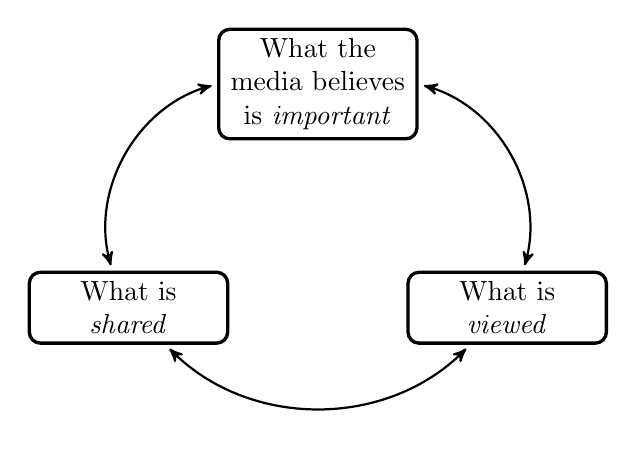
\begin{tikzpicture}[node distance=1cm, auto,]
 %nodes
 \node[punkt] (media) {What the media believes is \emph{important}};
 \node[below=2cm of media] (dummy) {};
 % We make a dummy figure to make everything look nice.
 \node[punkt,right=of dummy] (view) {What is \emph{viewed}}
   edge[pil,<->,bend right=45] (media.east); % edges are used to connect two nodes

 \uncover<2>{\node[punkt,left=of dummy] (share) {What is \emph{shared}}
   edge[pil,<->, bend left=45] (media.west)
   edge[pil,<->, bend right=45] node[auto] {} (view);}
\end{tikzpicture}
\end{center}
\end{frame}

\subsection{}
\begin{frame}{Data Overview}
\begin{itemize}
\item Scraped articles from \emph{New York Times} website between February 18 and April 28, 2015.
\item \emph{Article categories:} printed front page, digital front page (top, bottom \& opinion section), most viewed, most emailed, most shared on Facebook, most shared on Twitter
\item \emph{Extracted information:} title, author, date, time, URL, full text
\item \emph{Total number of unique articles:} 5504
\end{itemize}
\end{frame}

\subsection{}
\begin{frame}{Content of New York Times Articles}
\begin{itemize}
\item Summarize content using \emph{structural topic model} \citep{roberts2014structural,roberts2014stm}
\begin{itemize}
\item Each document is modeled as a \emph{mixture} of $K$ topics
\item \emph{Prevalence} of topics in documents can be influenced by a set of covariates
\item (Word use within each topic can be influenced by a set of covariates)
\end{itemize}
\item \emph{Number of topics}: 20
\end{itemize}
\end{frame}

\section{Results}

\subsection{}
\begin{frame} %[allowframebreaks]
  \frametitle{Topic Proportions}
  \begin{figure}
  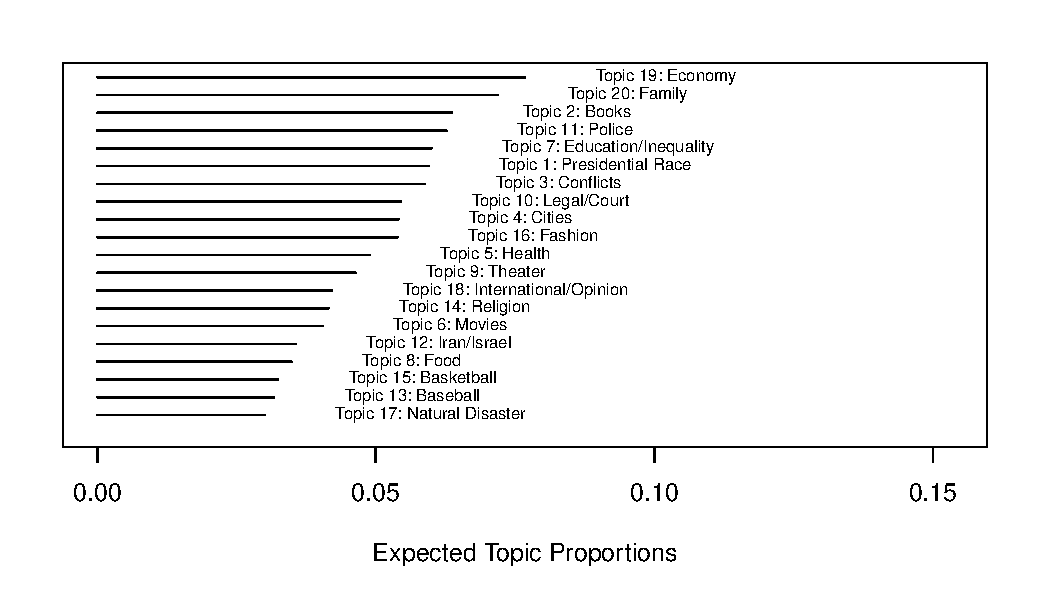
\includegraphics[width = \textwidth]{../calc/fig/prop.pdf}
  \end{figure}
\end{frame}

\subsection{}
\begin{frame} %[allowframebreaks]
  \frametitle{Example for Topic Perspectives}
  \begin{figure}
  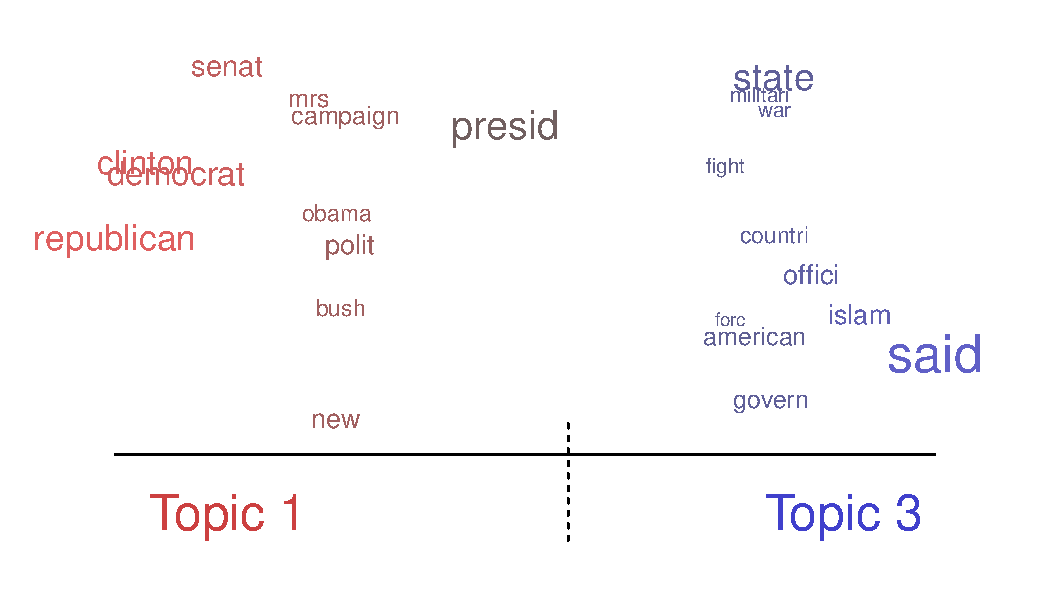
\includegraphics[width = \textwidth]{../calc/fig/perspective.pdf}
  \end{figure}
\end{frame}

\subsection{}
\begin{frame} %[allowframebreaks]
  \frametitle{Changes in Topic Distributions (Newspaper Section)}
  \begin{figure}
  \only<1>{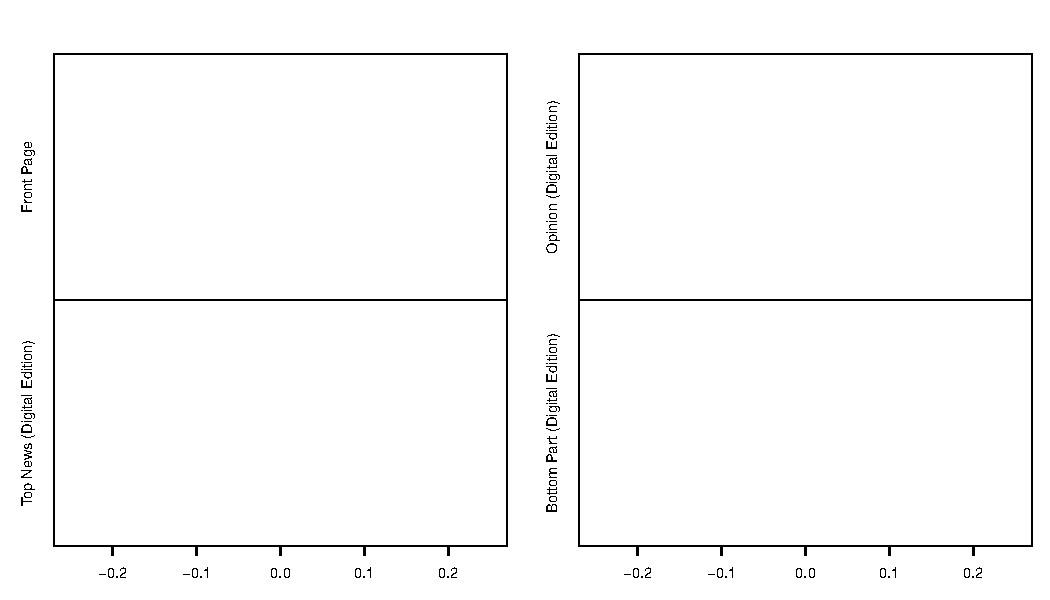
\includegraphics[width = \textwidth]{../calc/fig/res_nyt_polecon_empty.pdf}}
  \only<2>{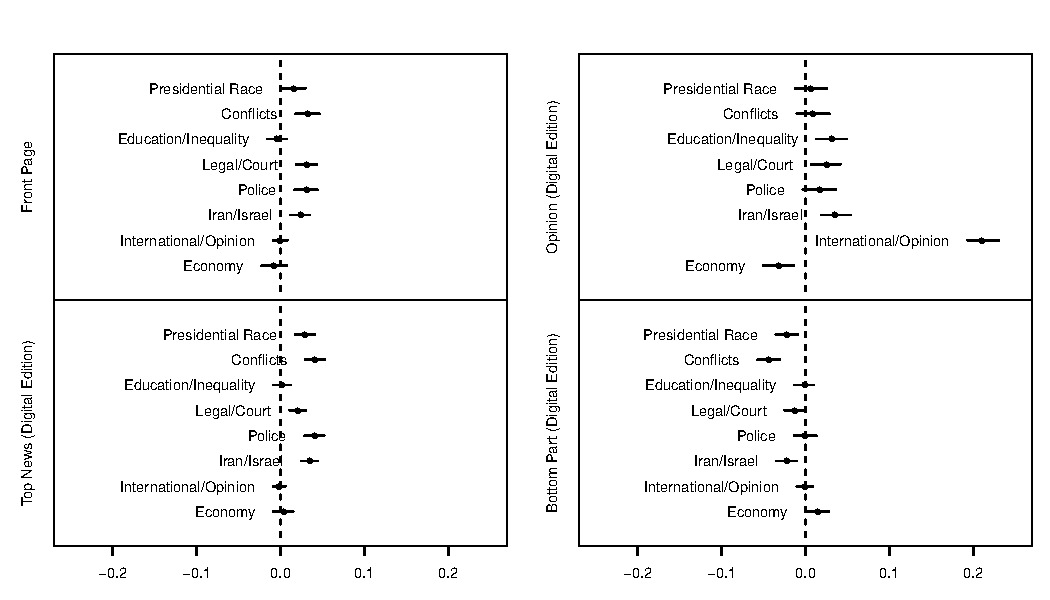
\includegraphics[width = \textwidth]{../calc/fig/res_nyt_polecon.pdf}}
  \end{figure}
\end{frame}

\subsection{}
\begin{frame} %[allowframebreaks]
  \frametitle{Changes in Topic Distributions (Shared/Viewed)}
  \begin{figure}
  \only<1>{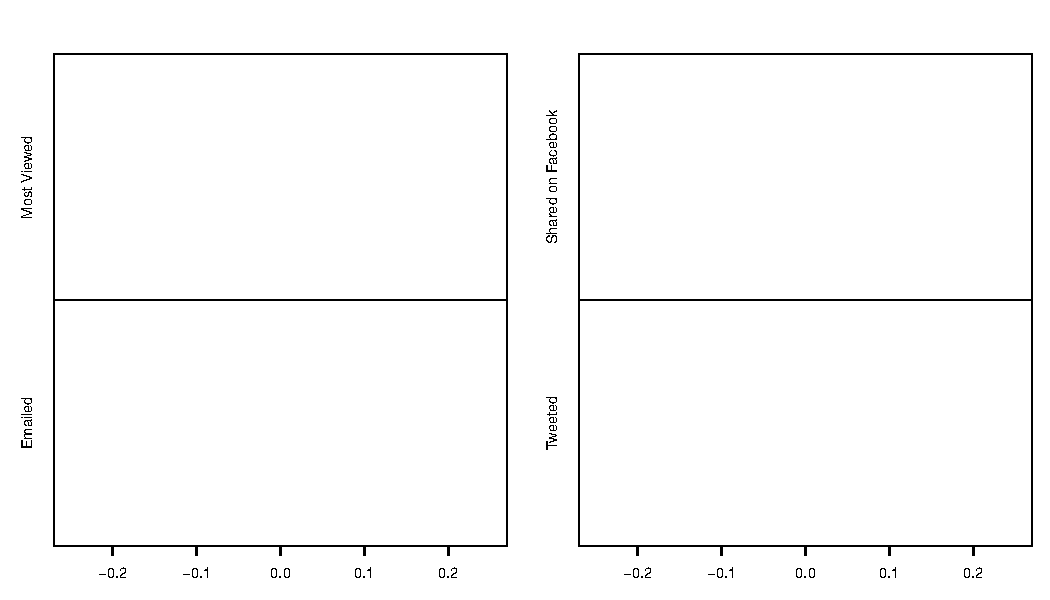
\includegraphics[width = \textwidth]{../calc/fig/res_share_polecon_empty.pdf}}
  \only<2>{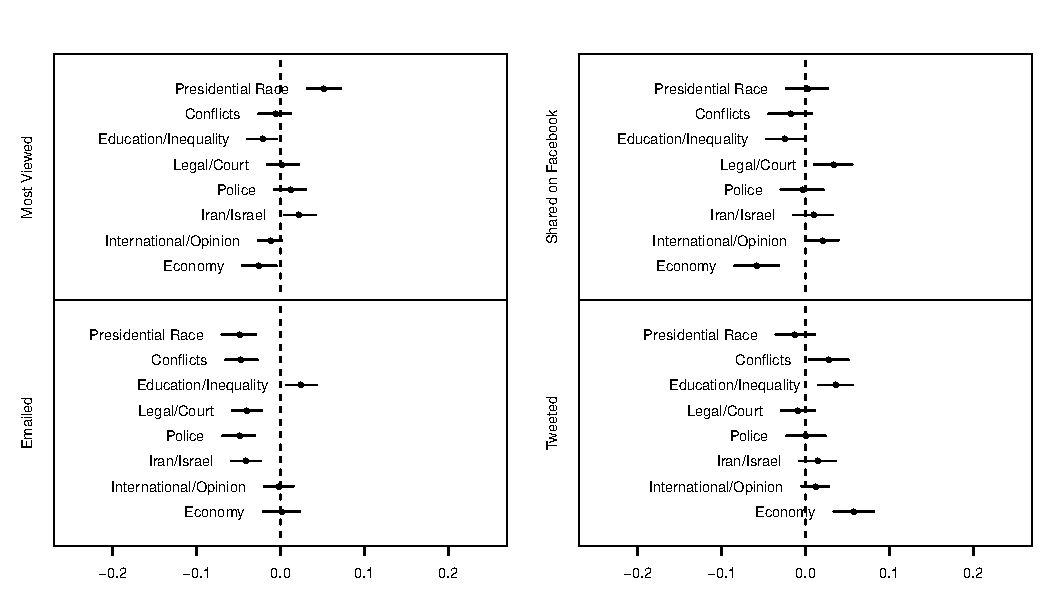
\includegraphics[width = \textwidth]{../calc/fig/res_share_polecon.pdf}}
  \end{figure}
\end{frame}

\subsection{}
\begin{frame} %[allowframebreaks]
  \frametitle{Topic Proportions over Time (Newspaper Section)}
  \begin{figure}
  \only<1>{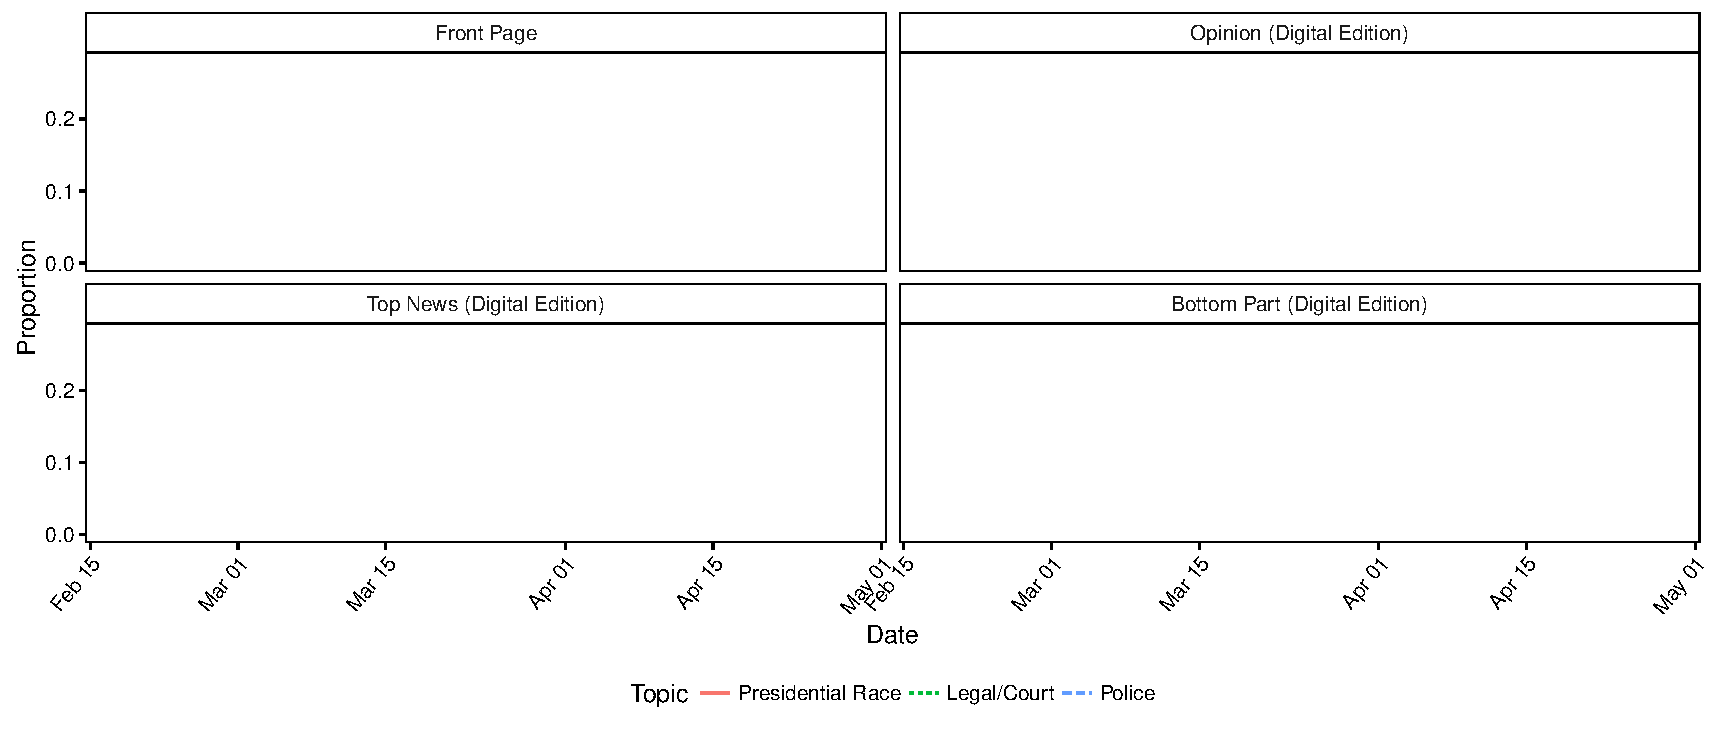
\includegraphics[width = \textwidth]{../calc/fig/series_nyt_main_empty.pdf}}
  \only<2>{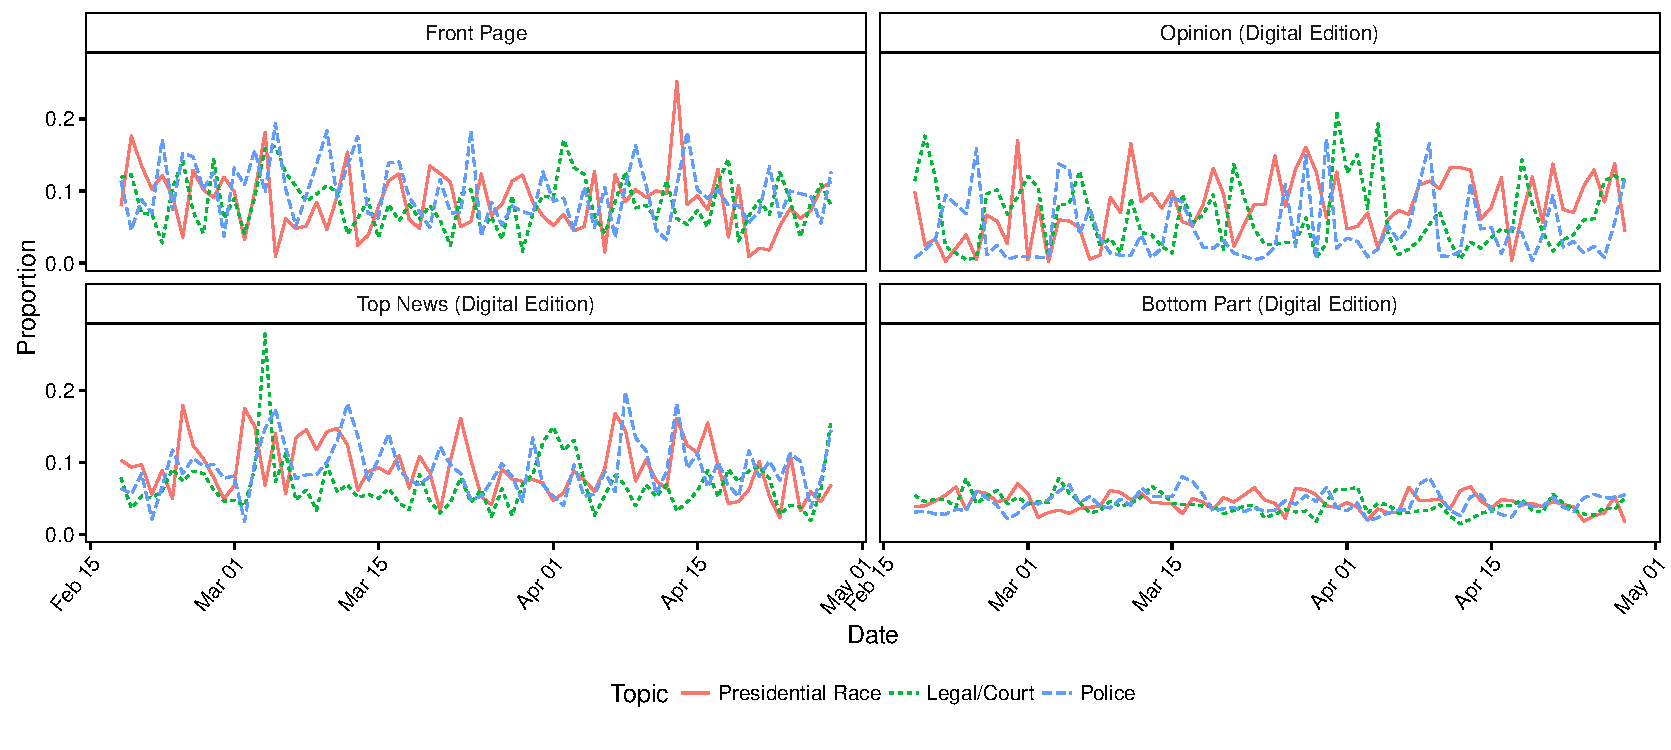
\includegraphics[width = \textwidth]{../calc/fig/series_nyt_main.pdf}}
  \end{figure}
\end{frame}

\subsection{}
\begin{frame} %[allowframebreaks]
  \frametitle{Topic Proportions over Time (Shared/Viewed)}
  \begin{figure}
  \only<1>{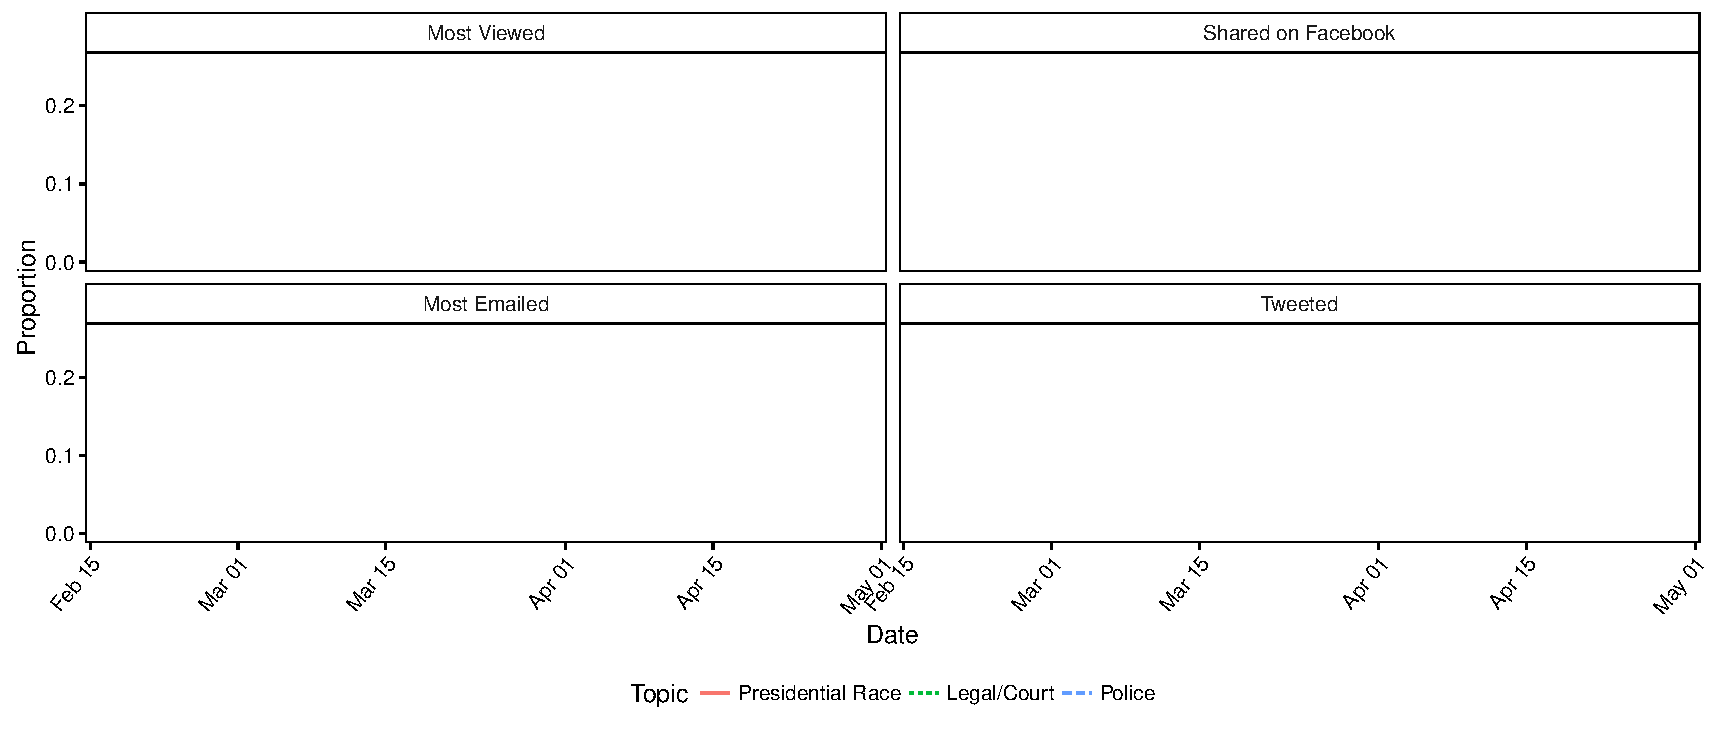
\includegraphics[width = \textwidth]{../calc/fig/series_share_main_empty.pdf}}
  \only<2>{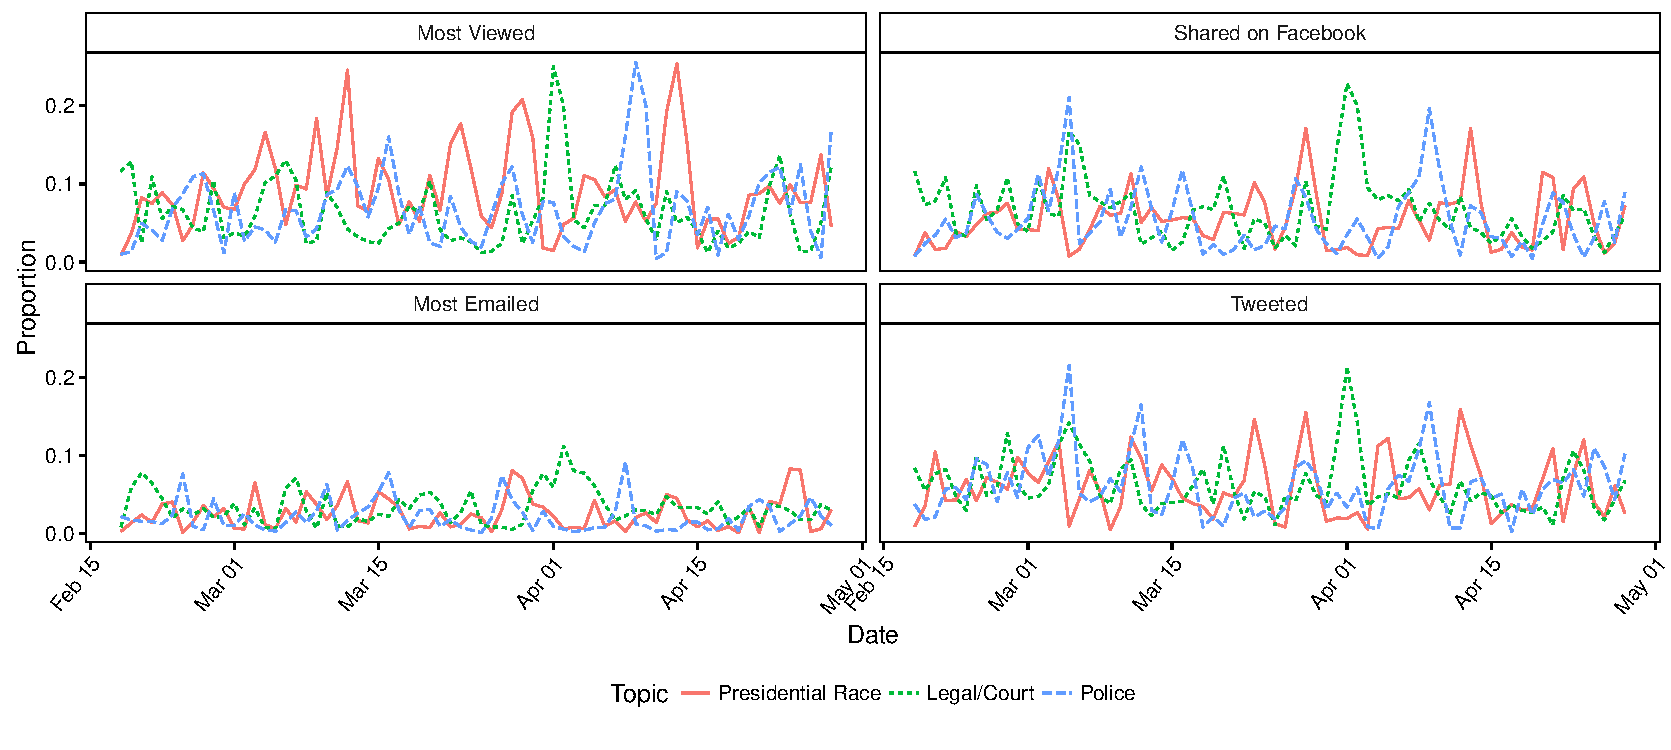
\includegraphics[width = \textwidth]{../calc/fig/series_share_main.pdf}}
  \end{figure}
\end{frame}

\subsection{}
\begin{frame} %[allowframebreaks]
  \frametitle{Article Readability by Category}
  \begin{figure}
  \only<1>{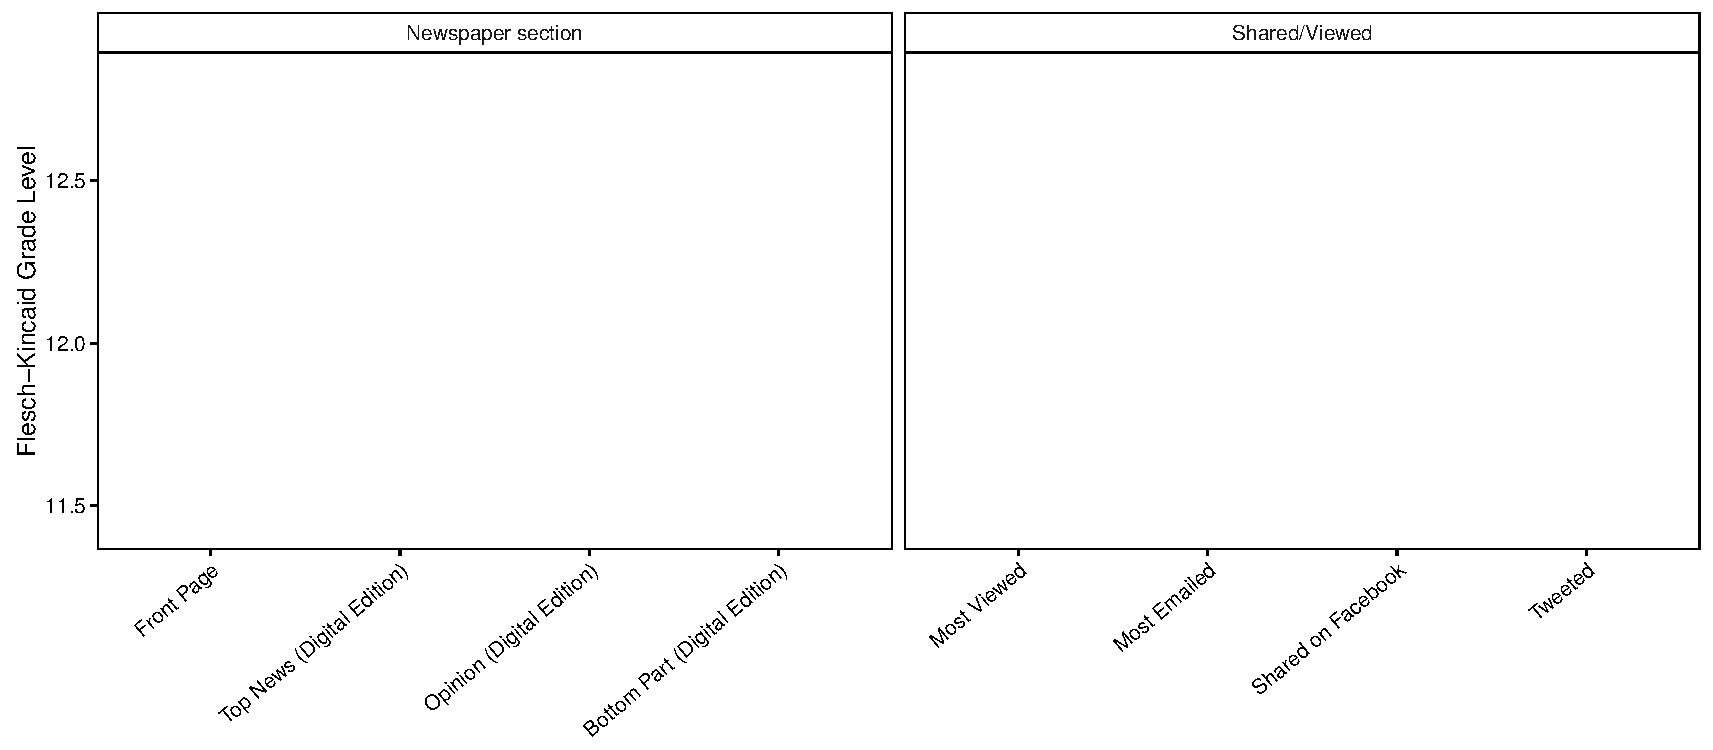
\includegraphics[width = \textwidth]{../calc/fig/readability_empty.pdf}}
  \only<2>{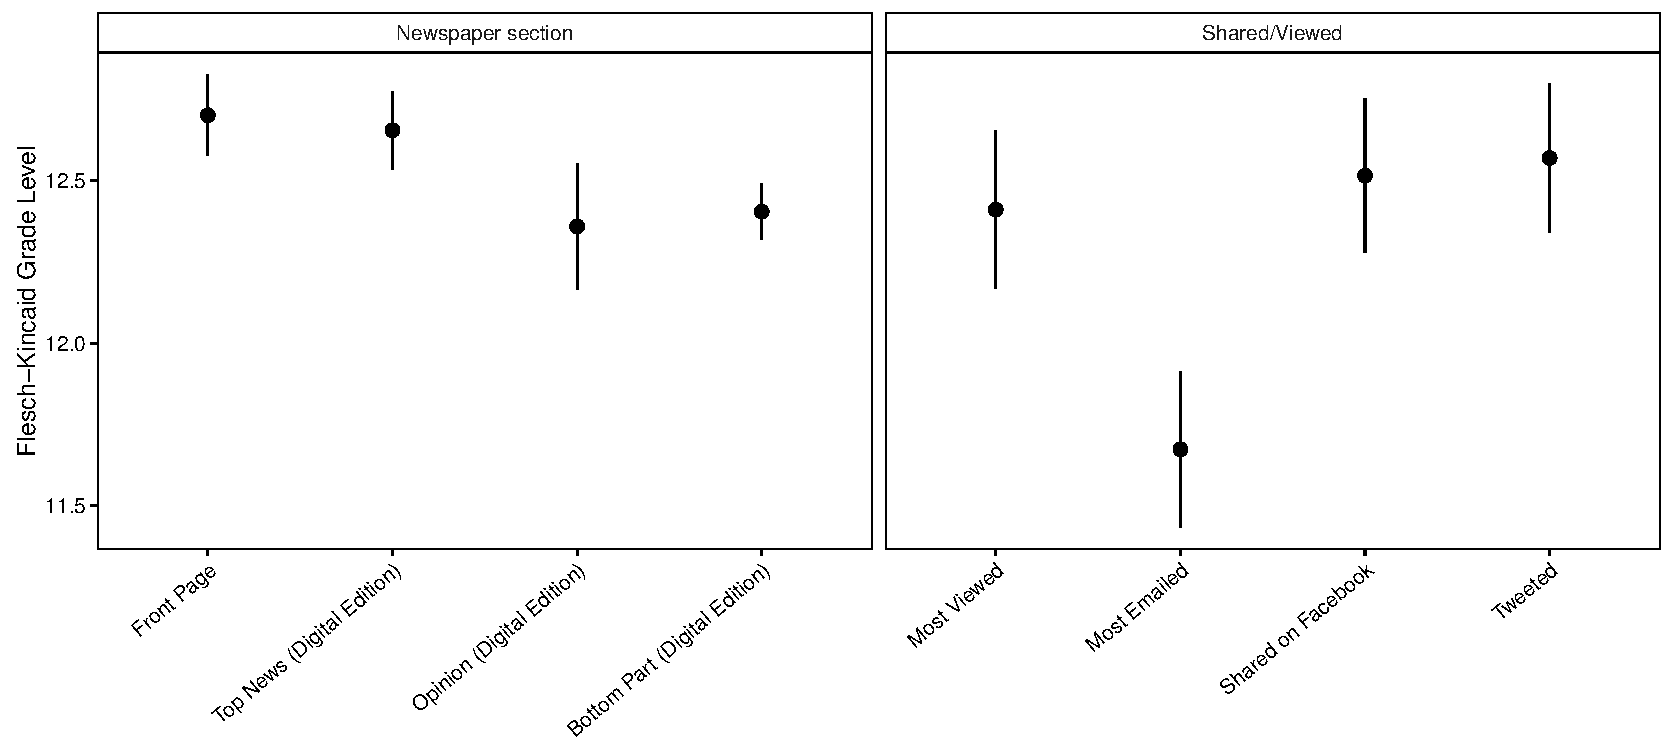
\includegraphics[width = \textwidth]{../calc/fig/readability.pdf}}
  \end{figure}
\end{frame}

\subsection{}
\begin{frame} %[allowframebreaks]
  \frametitle{What stays in the loop?}
  \begin{figure}
  \only<1>{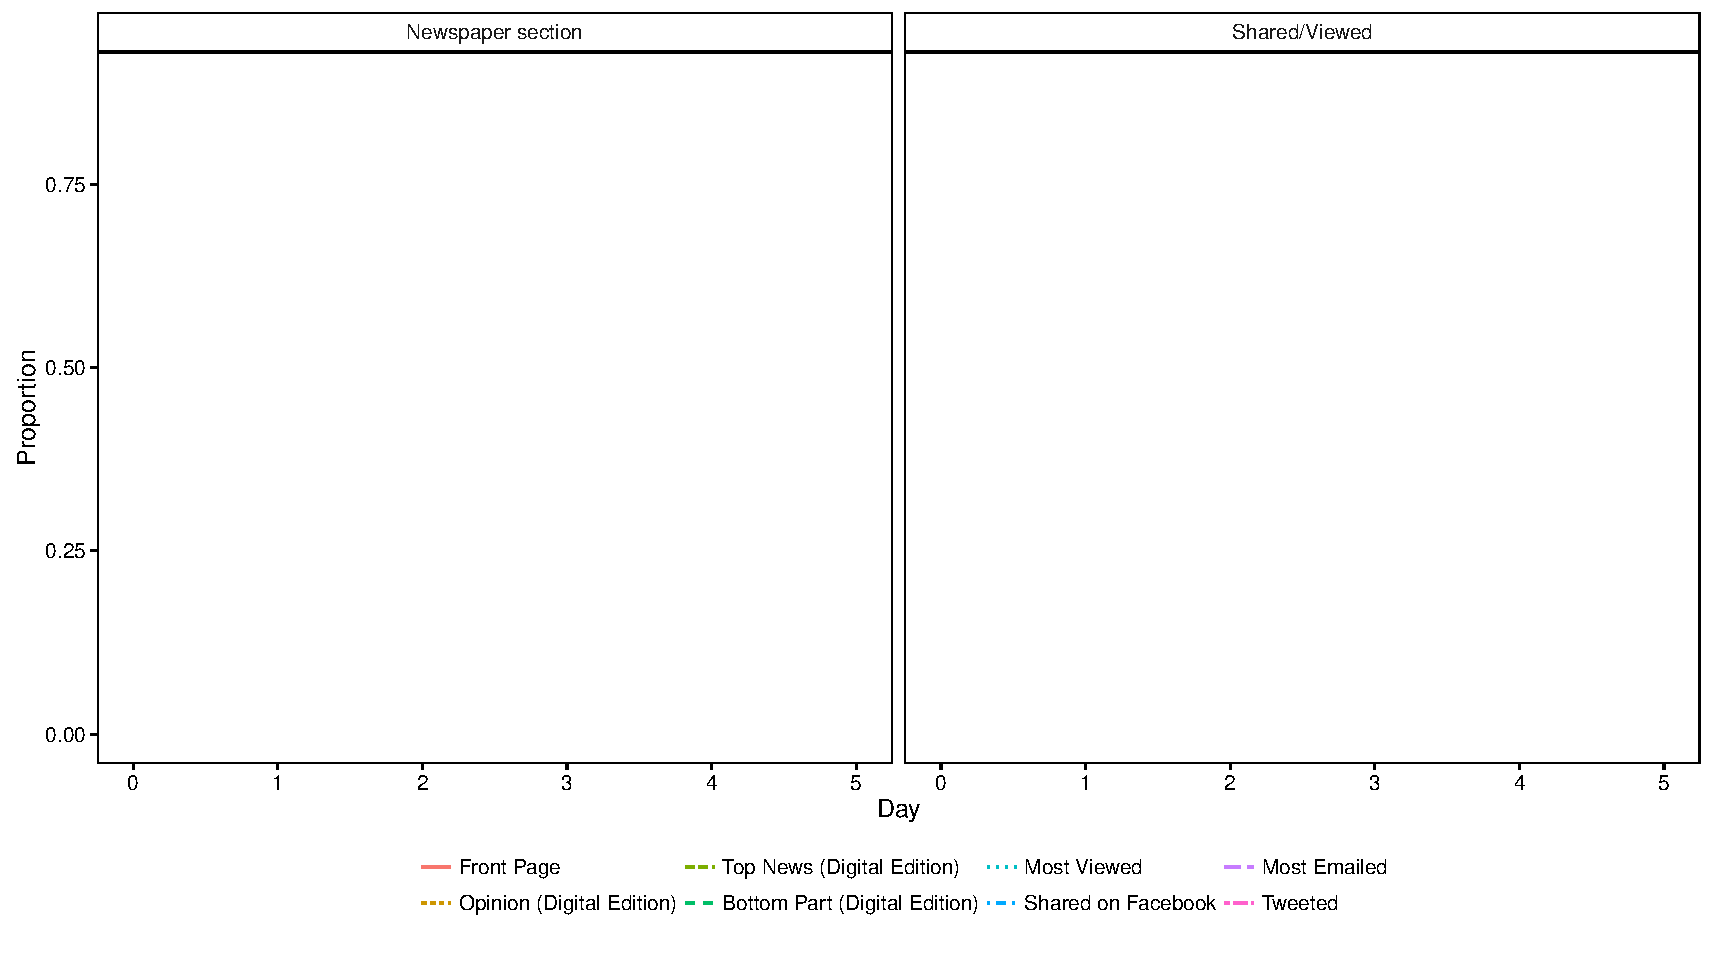
\includegraphics[width = \textwidth]{../calc/fig/switch_empty.pdf}}
  \only<2>{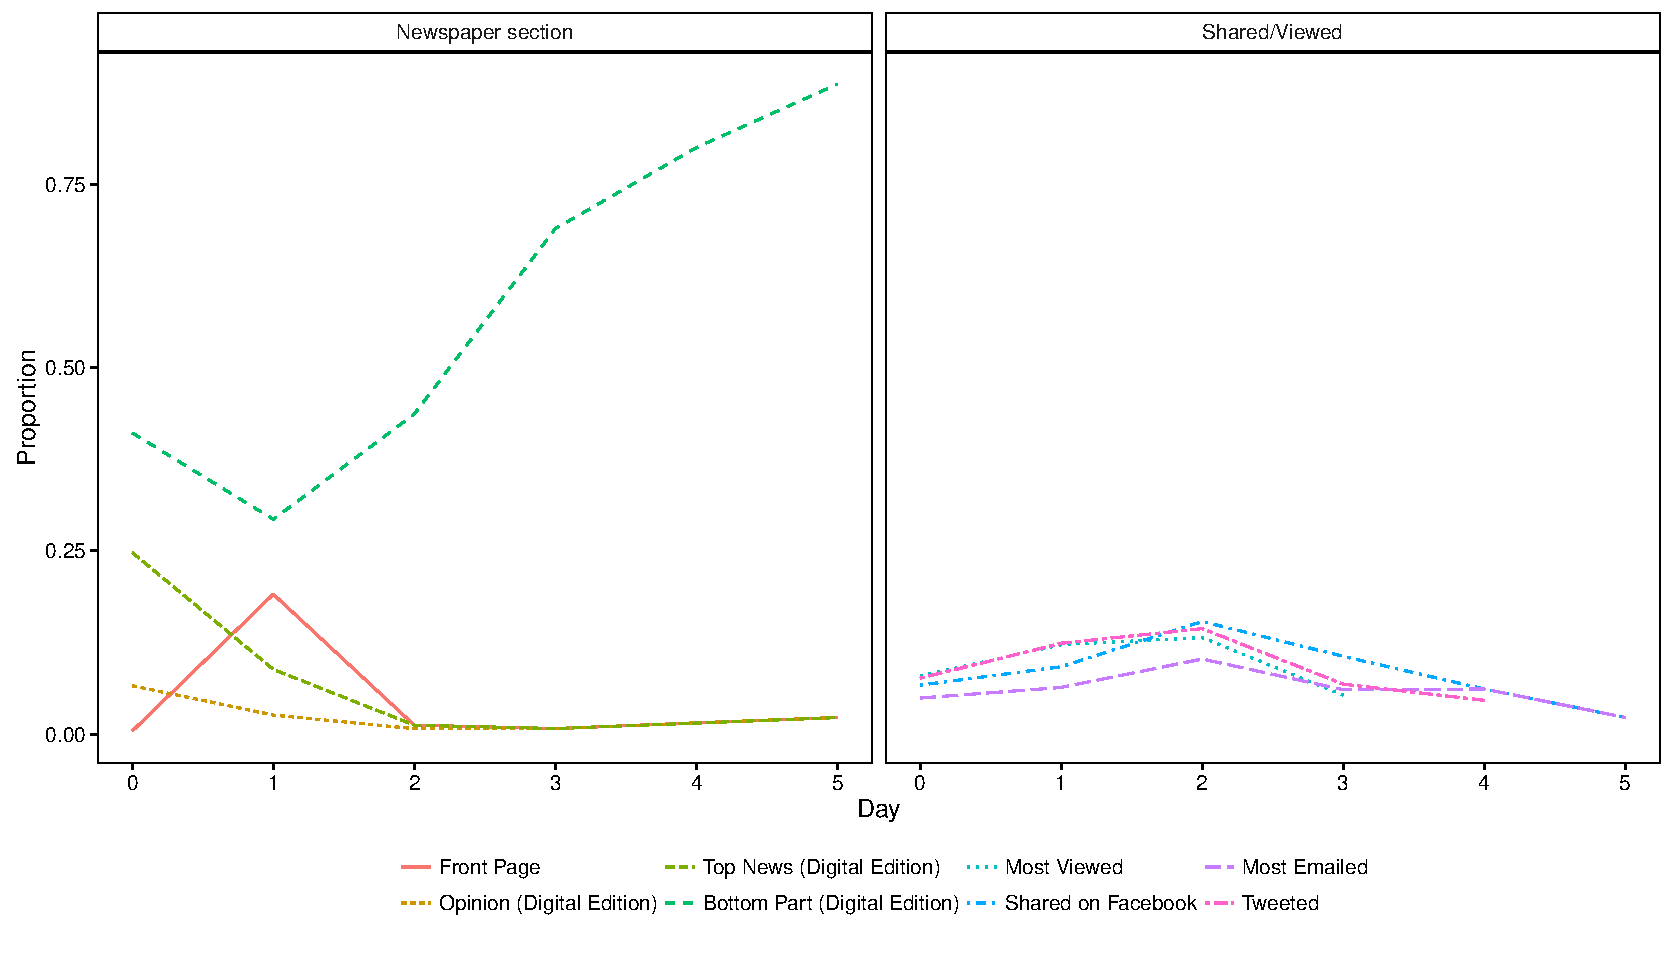
\includegraphics[width = \textwidth]{../calc/fig/switch.pdf}}
  \end{figure}
\end{frame}


\section{Conclusion}
\subsection{}
\begin{frame}%[allowframebreaks]
  \frametitle{Conclusion}
  \begin{itemize}
\item There are differences in types of articles that are shared across media, as well as articles that the \emph{New York Times} places on its front page
\begin{itemize}
\item Disagreement on importance of certain news stories
\end{itemize}
\item \emph{Limitations:}
\begin{itemize}
\item Reader of the New York Times may be different than readers of other news sources.
\item The editorial team of the New York times may be less influenced by social media than other news outlets.
\end{itemize}
\item \emph{Subsequent analyses:}
\begin{itemize}
\item Closer analysis of temporal development of articles, track how long articles remain popular in a given cycle
\item Matching individual articles to broader news stories
\item Take into account additional meta information (length etc.)
\end{itemize}
  \end{itemize}
\end{frame}

\subsection{}
\begin{frame}%[allowframebreaks]
  \begin{center}
  \large{Thank you very much for your attention!}\\ \vspace{2em}
  Comments, questions?\\
  \emph{\texttt{patrick.kraft@stonybrook.edu}}
  \end{center}
\end{frame}

\section{Appendix}
\subsection{}
\begin{frame}%[allowframebreaks]
  \frametitle{Topic Words I}
  \begin{figure}
  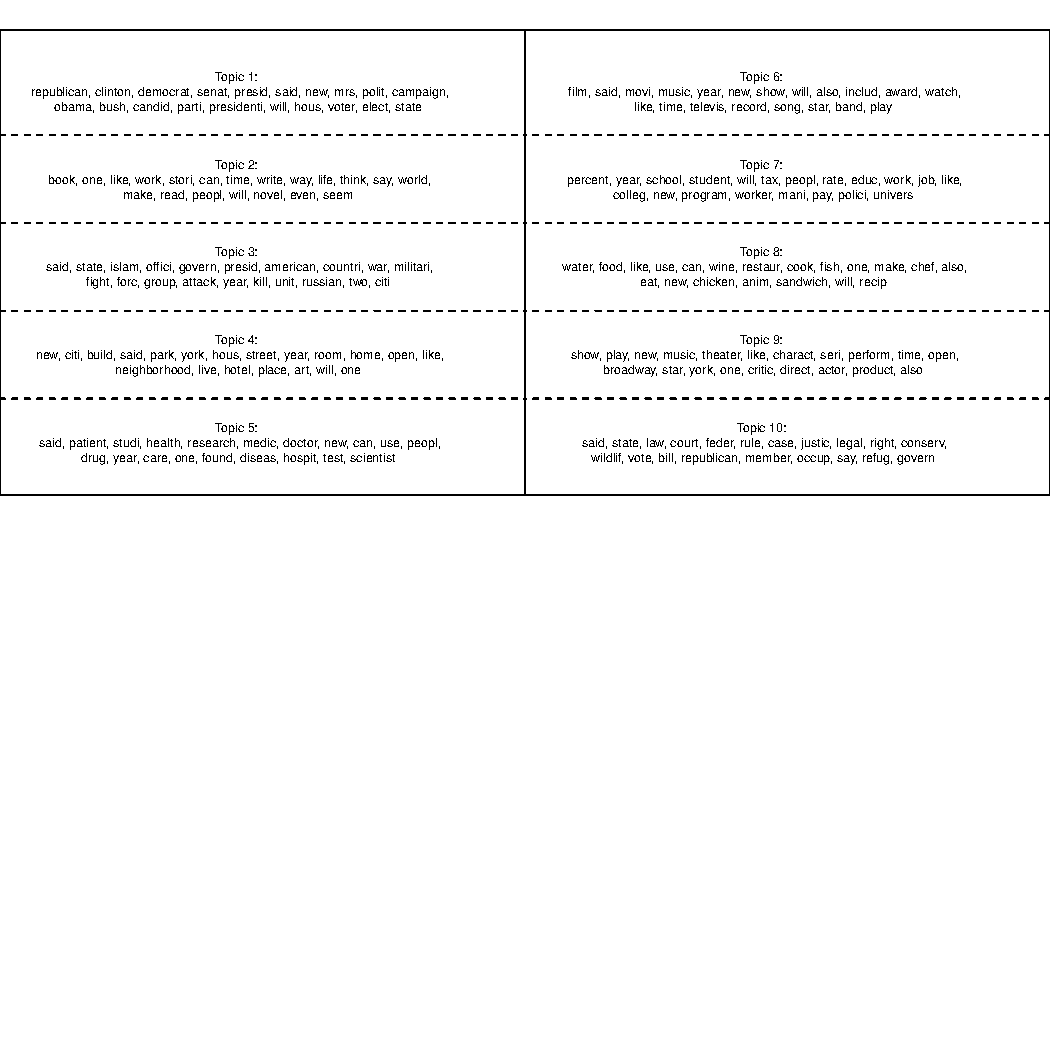
\includegraphics[width = \textwidth]{../calc/fig/words_top.pdf}
  \end{figure}
\end{frame}

\begin{frame}%[allowframebreaks]
  \frametitle{Topic Words II}
  \begin{figure}
  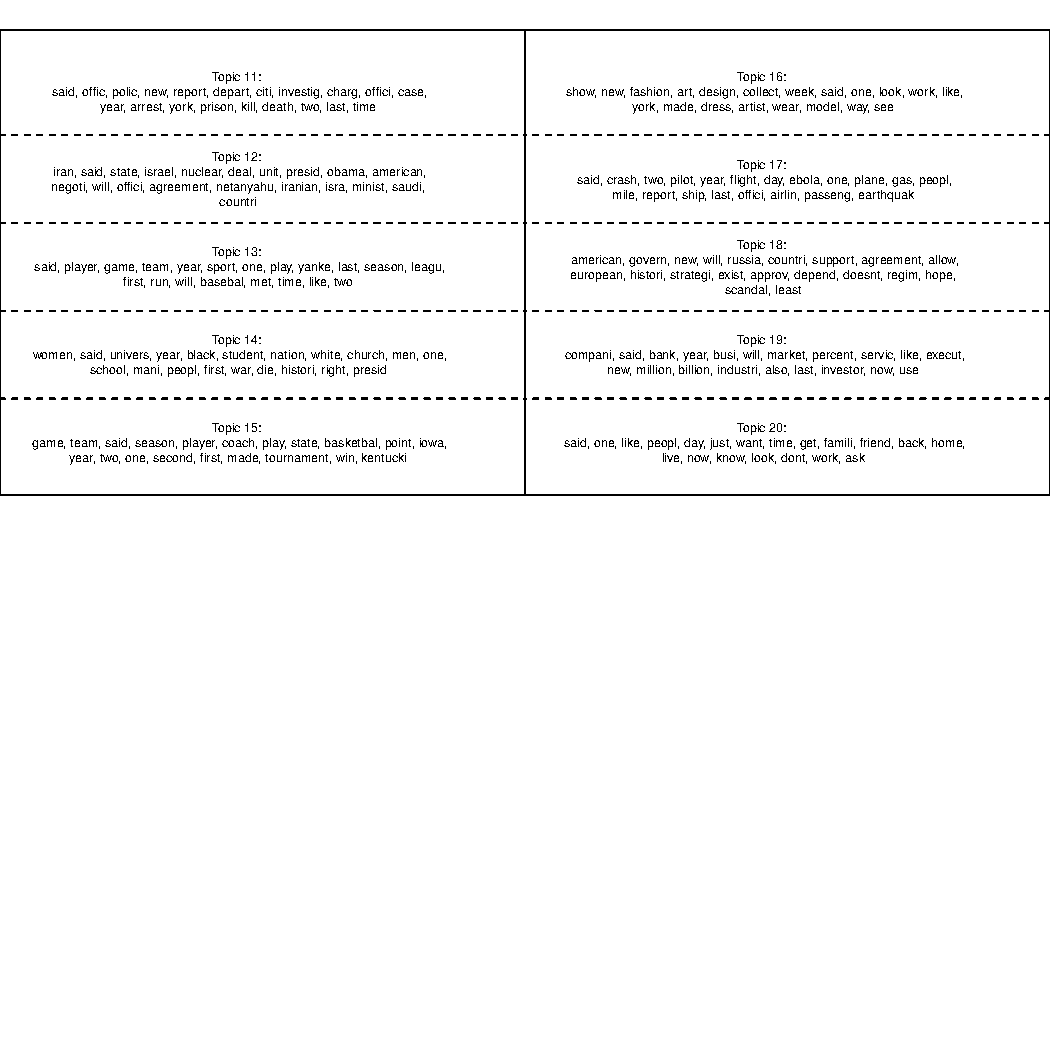
\includegraphics[width = \textwidth]{../calc/fig/words_bottom.pdf}
  \end{figure}
\end{frame}

\subsection{}
\begin{frame} %[allowframebreaks]
  \frametitle{Changes in Topic Distributions (Newspaper Section)}
  \begin{figure}
  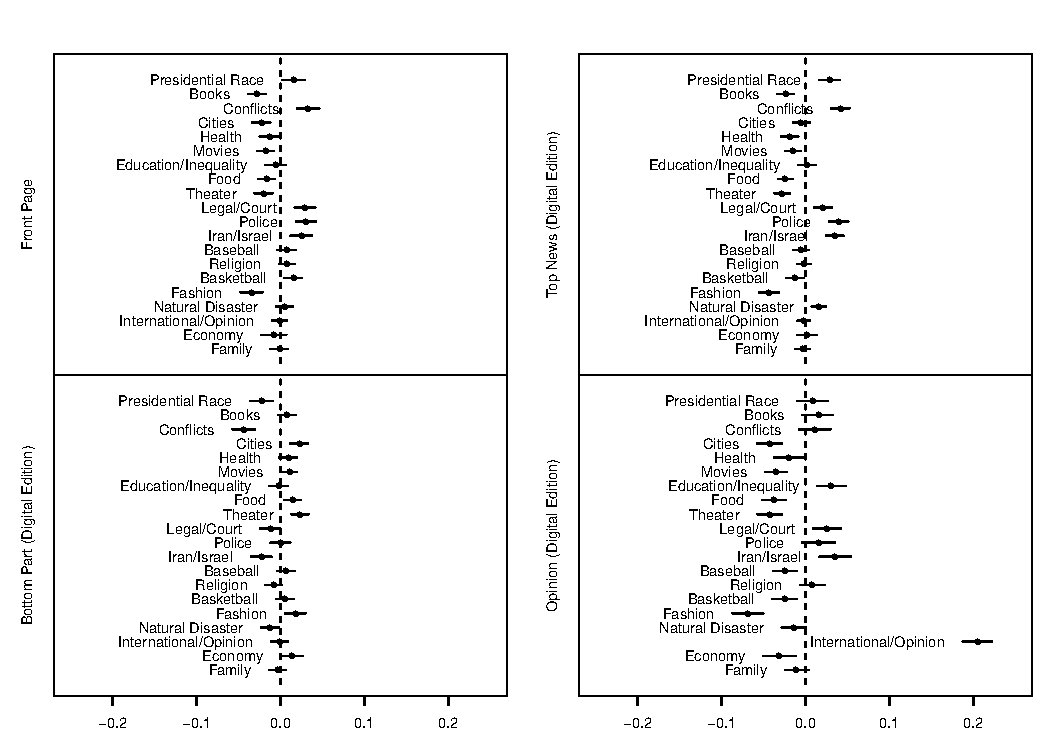
\includegraphics[width = .85\textwidth]{../calc/fig/res_nyt.pdf}
  \end{figure}
\end{frame}

\subsection{}
\begin{frame} %[allowframebreaks]
  \frametitle{Changes in Topic Distributions (Shared/Viewed)}
  \begin{figure}
  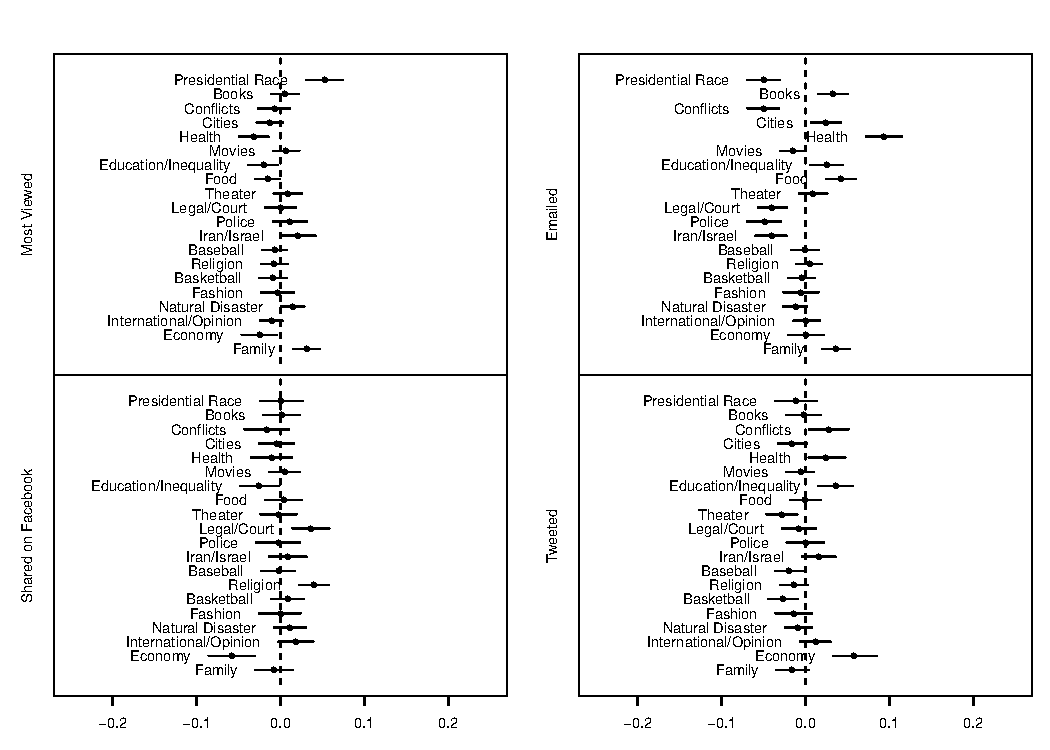
\includegraphics[width = .85\textwidth]{../calc/fig/res_share.pdf}
  \end{figure}
\end{frame}

\subsection{}
\begin{frame} %[allowframebreaks]
  \frametitle{Topic Proportions over Time (Newspaper Section)}
  \begin{figure}
	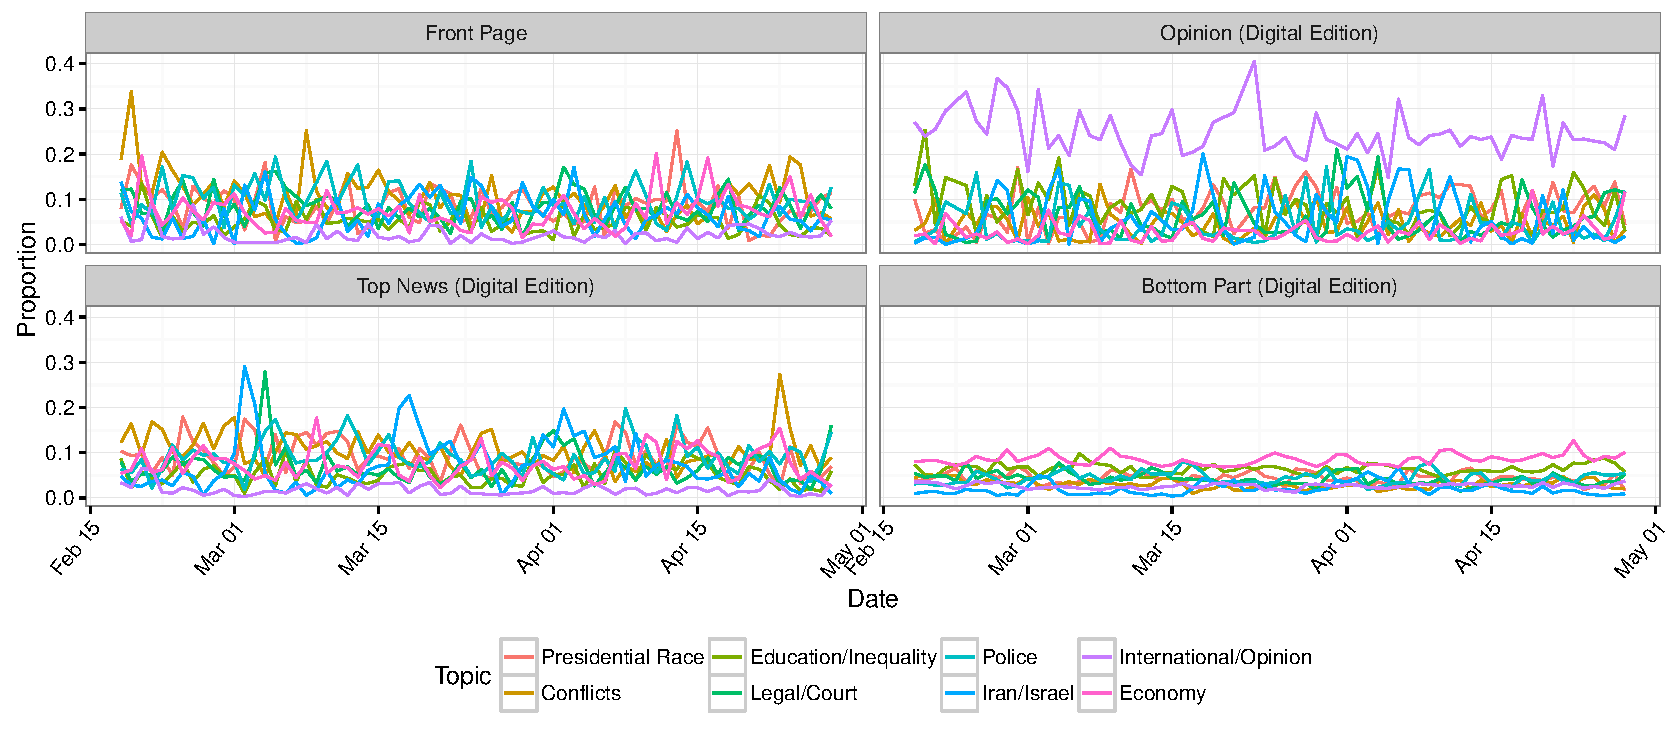
\includegraphics[width = \textwidth]{../calc/fig/series_nyt.pdf}
  \end{figure}
\end{frame}

\subsection{}
\begin{frame} %[allowframebreaks]
  \frametitle{Topic Proportions over Time (Shared/Viewed)}
  \begin{figure}
  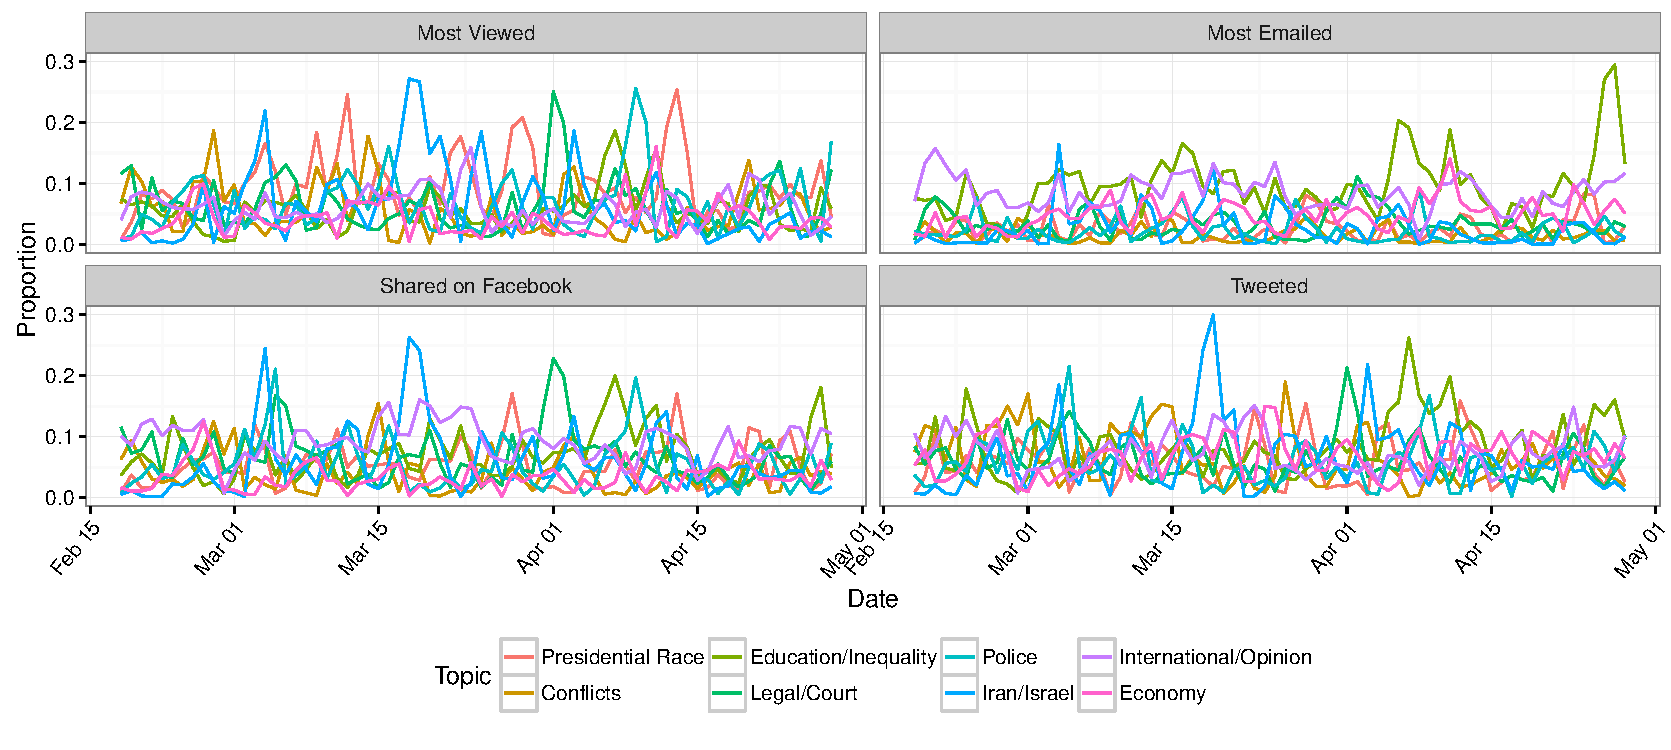
\includegraphics[width = \textwidth]{../calc/fig/series_share.pdf}
  \end{figure}
\end{frame}


\subsection{}
\begin{frame}
  \frametitle{References}
  \def\newblock{\hskip .11em plus .33em minus .07em}
  %\nocite{*}
  \begin{scriptsize}
    \bibliographystyle{../paper/apsr2006}
    \bibliography{../paper/JBRReferences.bib}
  \end{scriptsize}
\end{frame}

\end{document}